%!TEX TS-program = xelatex
\documentclass[]{friggeri-cv}
\addbibresource{bibliography.bib}
\usepackage{fontawesome}  
\usepackage{graphicx}
\usepackage{enumitem}
\graphicspath{ {images/} }

\begin{document}
\header{miruna}{popa}
       {data scientist}

% In the aside, each new line forces a line break
\begin{aside}
  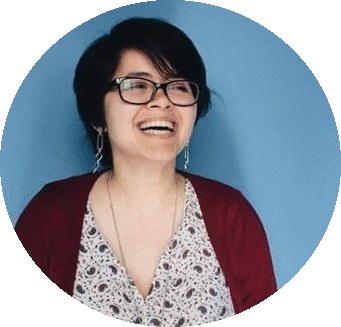
\includegraphics[width = 3cm, height = 3cm, keepaspectratio=true]{imageedit_3_7763302292.png}
  ~
  \section{about}
  ~
    Zehdenicker Str. 15
    10119 Berlin
    Deutschland
    ~
    {24 years old}
    {\color{lightgray} \faEnvelope \href{mailto:miruna.c.popa@gmail.com} {  miruna.c.popa\\@gmail.com}}
    {\color{lightgray} \faMobilePhone {  +4917656977157}}
    ~
    {\color{lightgray} \faGithub \href{https://www.github.com/mirunapopa} {  mirunapopa}}
    {\color{lightgray} \faLinkedin \href{https://www.linkedin.com/in/mirunapopa}{   mirunapopa}}
    ~
  \section{languages}
    romanian (native)
    english (fluent)
    german (beginner)
    spanish \& french notions
  ~
  \section{programming}
    {\color{red}  \faHeart { Python, Spark Scala, PostgreSQL}}
    {Google Spreadsheets, Command Line, Redshift}
    {Fiddled with: SAS, Systat, HTML, CSS, Latex}
  ~
  \section{graphic design}
    {Fiddled with Adobe Suite (Illustrator, Indesign, Photoshop)}
\end{aside}

\section{summary}

Experienced in startup scenes, working closely with managemnt in the company, eager to bring data closer to the rest of the company and to nourish a data driven mentality. Seeking challenging environments with creative and curious people, a place from which one never stops learning. 

\section{education}

\begin{entrylist}
  \entry
  {2011-2014}
  {B.S. in Economic Cybernetics,\\ 
  Statistics and Informatics} % Degree
  {Academy of Economic Studies, Bucharest, Romania} % Institution
  {\emph{Final  Thesis:  Music  Recommendation  Web  App using  Collaborative Filtering Algorithm and Scala Programming Language}}

  \entry
  {2013–2014}
  {Erasmus Student in\\
  Computer Science\\
  and Economics}
  {West Pomeranian University of Technology,  Szczecin, Poland}
  {Topics Studied: Data Analysis \&  Machine Learning, Java Programming, Economic Analysis}
  
\end{entrylist}

\section{experience}

\begin{entrylist}
  \entry
    {2014 - Present}
    { EyeEm GmbH, Berlin}
    {Data Analyst}
    {\begin{itemize}
    \item handling internal requests, as well as improving the process
    \item providing data for both internal requests, as well as Board Presentations
    \item automating recurring reports
    \item preparing ETL jobs which would feed data to Chartio Dashboards
    \item created a slack bot which would answer some frequently asked questions
    %\item helped improving search experience through performance dashboards and suggested searches
    \end{itemize}}
  \entry
    {07-10 2013}
    {Softgames GmbH, Berlin}
    {Internship QA}
    {\begin{itemize}
    \item testing games on Java, Android, iOS, Blackberry
    \item developing ad campaigns based on KPIs
    \item new user funnel analysis
    \item working closely with product managers and external partners on the development of games
    \end{itemize}}
  \entry
    {02-04 2013}
    {Visionware Romania, Bucharest}
    {Practicing Student}
    {\begin{itemize}
    \item participated in trainings on .Net, SharePoint, Dynamics CRM
    \item offered some practical solutions to existing problems
    \end{itemize}}
  \entry
    {10-12 2012}
    {Sanoma Hearst, Bucharest}
    {Internship Marketing}
    {\begin{itemize}
    \item created presentations and e-banners for Esquire, FHM
    \item participated in  promotional concepts for advertising campaigns
    \end{itemize}}
\end{entrylist}

\pagebreak

\section{volunteering}

\begin{entrylist}
  \entry
  {2011-2013}
  {Volunteers for Ideas and Projects, Bucharest}
  {}
  {\begin{itemize}
  \item Marketing \& Sales Officer
  \item Art Direction Coordinator
  \item Organizer for Visual Playground, a graphical design school for students.
  \end{itemize}}

  \entry
  {2007-2011}
  {AntiDrug Consilium, Bacau}
  {}
  {\begin{itemize}
    \item Project Coordinator for around 10 projects
    \item awarded Volunteer of the Year in 2009
  \end{itemize}}
  
  \entry
  {2007-2010}
  {Ingenious Drama Festival, Bacau}
  {}
  {\begin{itemize}
    \item Chief of Magazine Department
    \item awarded Most active member of the Department
  \end{itemize}}

\end{entrylist}

\end{document}